%===========================================================
% MEMORY MAP SECTION
%===========================================================
\section{Memory Map Manager}
\label{sec:memmap}
%
Creating and enforcing protection domains is a challenging task on
resource constrained embedded platforms.
%
Initial SFI designs allowed a sandboxed module to access a single
contiguous range of memory~\cite{wahbe93sfi}.
%
Motes' limited physical memory and absence
of virtual memory precludes this partitioning; such a partition would
constrain applications by severely limiting available memory and lead
to internal fragmentation, extremely wasteful on severely resource
constrained platforms.
%
%% Static contiguous partitioning is only possible in desktop systems
%% with large address spaces~\cite{wahbe93sfi}.
%
Harbor's \emph{memory map} abstraction was designed with the following
requirements:
%
first, it should have a small and customizable memory footprint;
%
second, it should permit arbitrary layout of state within the data memory;
%
and third, it should be easy to incorporate into existing
operating systems.
%
We propose a design that satisfies these requirements.
%
%-----------------------------------------------------------------
\subsection{Data Structure}
%
We assume a sensor node's address space is partitioned by the operating
system into small, contiguous \emph{blocks} of equal size, then allocated
to domains in \textit{segments} consisting of sets of contiguous blocks.
%
(On AVR, SOS's block size is 8~bytes.)
%
The allocation of segments to domains could be static (at compile
time) or dynamic (through malloc).
%
A domain could be allocated multiple segments that are scattered
randomly across entire address space.
%
The Harbor memory map contains \emph{per-block} access permissions for
the entire address space.
%
The main operation of the memory map is to store and retrieve access
permissions for a given address.
%
Its design goal is to balance lookup efficiency and the extra storage
required for the permissions table.
%
The memory map contains ownership information (a domain identity) for every
block of memory, and encodes information about memory layout, such as
the start of a logical allocation segment.
%
The memory map must contain sufficient permission bits per block to encode
the total number of domains supported by the system.
%
Supporting two distinct domains (kernel and user) requires just one
domain bit per block, four domains require two domain bits per block,
and so forth.
%
Table~\ref{tab:mmap_table} shows an example of Harbor's memory map encoding
in a system with 8 domains.
%
\begin{table}[htdp]
\centering
\small{
\begin{tabular}{|c|l|}
	\hline
	Code & Meaning\\
	\hline
	1111 & Free, or start of kernel allocated segment\\
	1110 & Later portion of kernel allocated segment\\
	xxx1 & Start of user allocated segment\\
	xxx0 & Later portion of user allocated segment\\
	\hline
\end{tabular}}
\caption{Memory map information encoding for 8-domain protection.}
\label{tab:mmap_table}
\end{table}

%
The memory map is a configurable data structure; tradeoffs between
the inter-module protection and memory map size are discussed in
Section~\ref{sec:mmapdesignspace}.
%
%The design of memory map uses two bits of encoded information per
%block to provide memory protection.
%
%Due to the severe memory resource constraints, the memory map is
%designed to have a very small memory footprint. 
%
%The memory map is organized as a byte array where each byte is packed
%to store permission information about multiple blocks.
%
%Such an organization was chosen for maximum storage efficiency and
%minimum resource utilization.
%
%The memory protection mechanism intercepts every write operation of a
%user module to ensure that the permissions are not violated.
%
%The main task of the memory map manager is to store or retrieve the
%permissions for any given address.
%
%--------------------------------
\subsubsection{Address Translation}
\label{sec:memtrans}
%
Figure~\ref{fig:addr_memmap_translate} shows how an address is looked up in
the memory map.
%
Assuming a block size of 8 bytes, the last three bits of address are an
offset into a given block.
%
The remaining bits of the address represent a block number in data memory.
%
Access permissions are packed into a byte.
%
If encoded information is stored in four bits (for 8-domain
protection), then each byte would contain information for two
contiguous memory blocks.
%
Therefore, the last bit of block number selects a memory map record
from within an access permissions byte.
%
The remaining bits of the block number form an index into the memory map table.
%
This design was chosen to minimize memory footprint.
%
\begin{figure}[htbp]
  \centering
  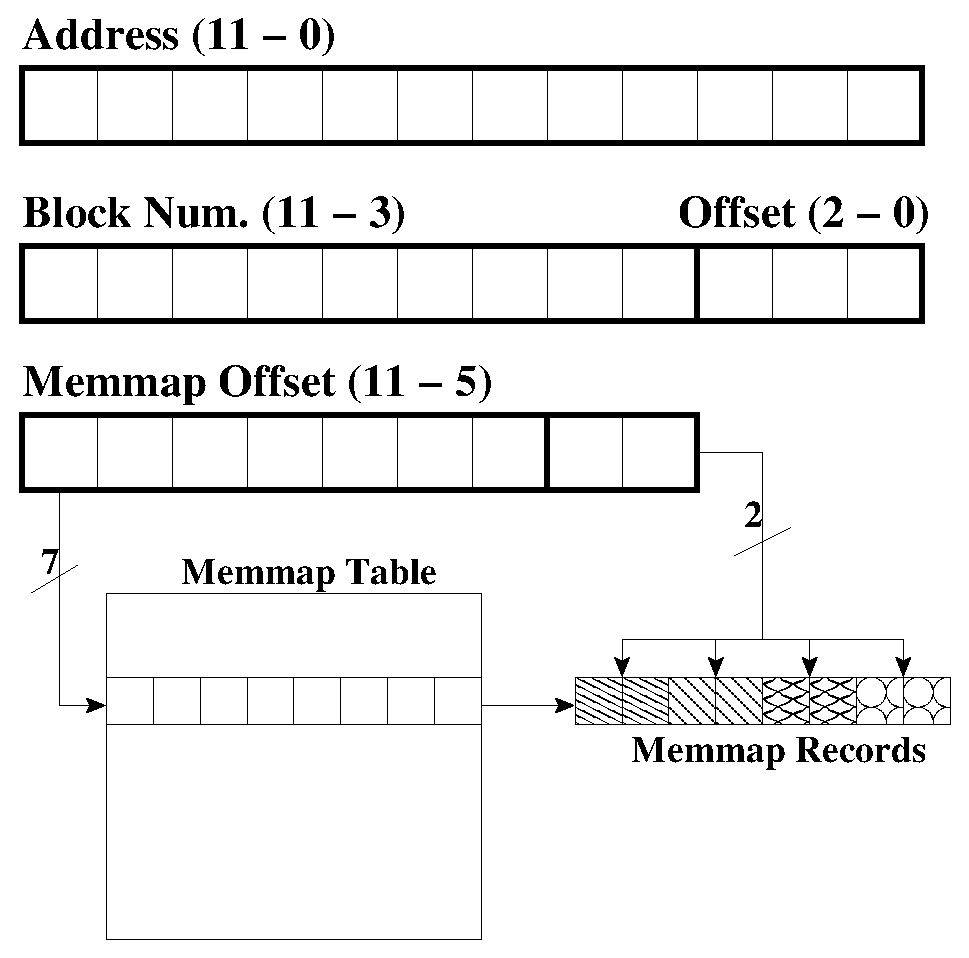
\includegraphics[height=2.0in,
  keepaspectratio=true]{figures/memaddrtrans.eps}
  \caption{Address to memory map translation (8-domain mode)}
  \label{fig:addr_memmap_translate}
\end{figure}
%
%------------------------------
\subsubsection{Memory Map API}
%
The memory map data structure and address translation operations are
encapsulated in an object accessible through the API
in Table~\ref{tab:memmap_api}. 	
%
%
% If we optimize the memory map table to not include certain portions
% of the address space, then what will happen if we accidentally pass
% an unmapped address ?
%
%
%
\begin{table}[htdp]
   \centering
   \small{
   \begin{tabular}{|l|}
   \hline
   Prototype and Description \\
   \hline
   \texttt{int8\_t memmap\_set(uint8\_t blkID, uint8\_t nBlks, uint8\_t
   domID)}\\
   Set owner of segment [BlkID, BlkID + nBlks) to domID \\
   \hline
   \texttt{uint8\_t memmap\_get(uint8\_t blkID)}\\
   Get owner and layout of block number BlkID \\
   \hline
   \end{tabular}
   }
   \centering
   \caption{Memory map API}
   \label{tab:memmap_api}
\end{table}
%
%
%========================================================================================================================================
% MEMORY MAP CHECKER
%========================================================================================================================================
\subsection{Memory Map Checker}
\label{sec:mmapchecker}
%
Harbor's run-time checks validate memory accesses, in particular writes.
%
These accesses are validated using a protection model.
%
Our memory map checker enforces the protection model described earlier:
each user module can write only into its own domain.
%
% Further, a single trusted domain in the system is allowed to access all memory.
%
The memory map checker belongs to the trusted domain.
%
%A run-time checker restricts the memory access of user modules to permissible regions.
%
%The access control permissions are stored and tracked by the memory map manager.
%
%The policy used for access control can vary.
%
%The most common policy is to prevent the user modules from ever writing to a memory region that is owned by the kernel.
%
%The modules are instrumented to introduce checks before every write operation that needs protection.
%
%   // Get permissions through bit shifts
%   // uint8_t perms_bm = (BLOCK_TYPE_BM << ((mmap_offset >> 3) << 1));
Pseudocode for a write access check in a system with 8-domain protection is shown in Figure~\ref{fig:checker}.
%
\begin{figure} [htbp]
  \centering
  \begin{tiny}
\begin{verbatim}
write_access_check(addr_t addr, data_t data) {
   // Check is for writes outside stack region
   if (addr < STACK_PTR) {
      // Address translation: Get table index
      uint16_t blk_num = (addr >> log2_blk_size);
      uint16_t mmap_index = (blk_num >> log2_rec_per_byte);
      // Retrieve memory map byte
      uint8_t mmap_byte = MEM_MAP_PERMS_TBL[mmap_index];
  
      // Get the appropriate record in byte
      if (blk_num & SWAP_MASK) swap(mmap_byte);
      uint8_t mmap_owner = mmap_byte & OWNER_MASK;
      uint8_t first_blk_in_segment = mmap_byte & 1;

      // Validate access
      if (mmap_owner != curr_dom_id
          || (first_blk_in_segment && addr points to block metadata))
         mem_access_exception();

      // Perform store
      st addr, data;
   } else {
      // Check for writes to stack 
      stack_access_check(addr, data);
   } 
}
\end{verbatim}
      \end{tiny}
  \vskip-\baselineskip
  \caption{Pseudocode for Memory Map Checker (8-domain protection)}
  \label{fig:checker}
\end{figure}
%

The write access checker performs three operations.
%
First, it performs address translation to retrieve the byte containing
ownership information from the memory map table for a given address.
%
Second, it locates the appropriate record within that byte and determines
the domain of the block's owner.
%generates a bit mask from the address offset to derive the actual permission.
%
Third, it compares this domain ID and the current executing user module's domain ID.
%
A store is allowed only if these domains match.
%
As mentioned previously, the memory map manager does not maintain
permissions for run-time stack;
%
write accesses to the run-time stack are subject to a different
check described in Section~\ref{subsec:stackguard}.
%

%
\begin{figure}[htpb]
 \centering
  \mbox{
    \subfigure[Memory map byte for two
    domains]{\label{fig:memmaptwodoms}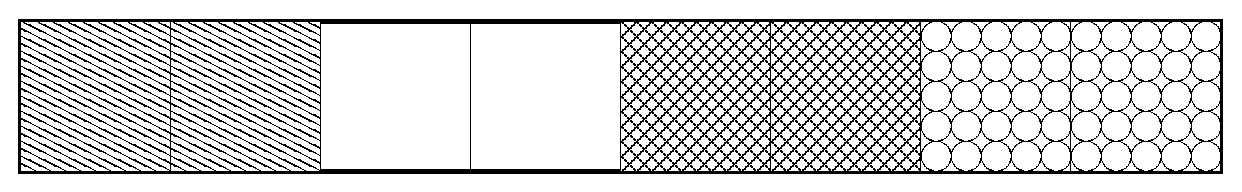
\includegraphics[width=2in,
      keepaspectratio = true]{figures/memmaptwodoms.eps}}
    \hspace{0.2in}
    \subfigure[Bit-Mask Lookup
    Table]{\label{fig:perm_lut}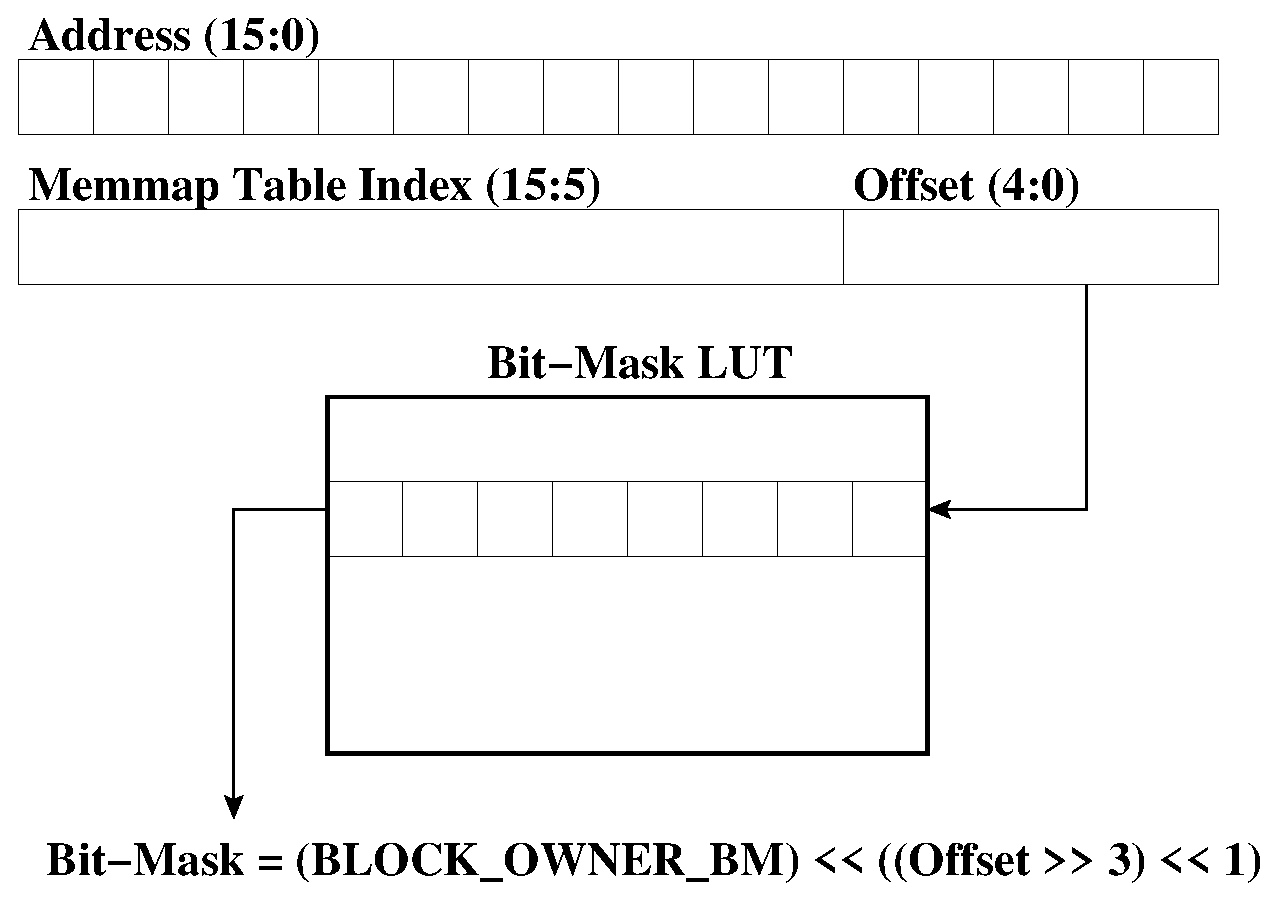
\includegraphics[height=1.5in,
      keepaspectratio = true]{Figures/perms_lut_opt.eps}}
  }
  \caption{Memory Map Checker Optimizations (2-domains)}
\end{figure}   
%
% \begin{figure}[htbp]
%   \centering
%    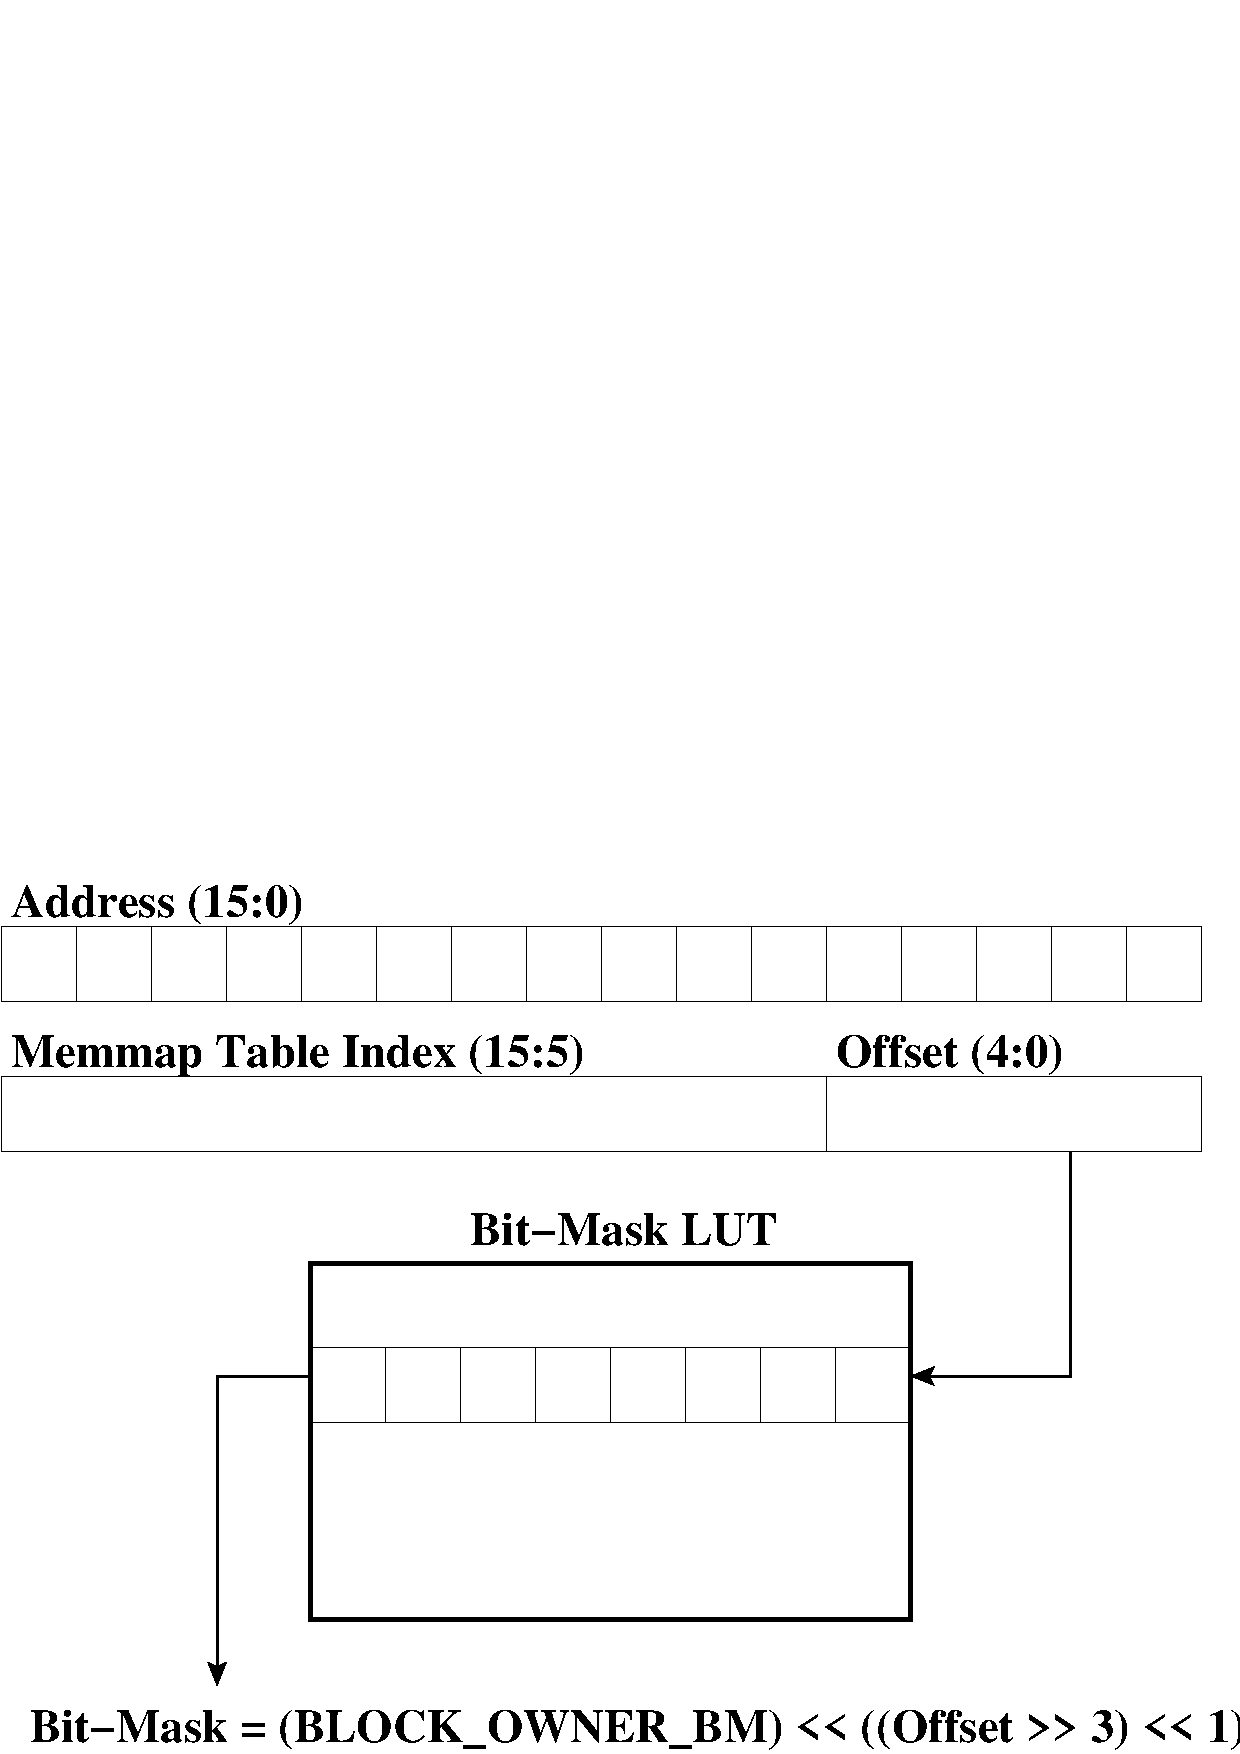
\includegraphics[height=1in, keepaspectratio=true]{figures/perms_lut_opt.jpg} 
%    \caption{Lookup table optimization to implement bit-shift operations}
%    \label{fig:perm_lut}
% \end{figure}
%
%-----------------------------------------
\subsubsection{Bit-Mask Lookup Table}
\label{sec:bitmasklut}
%
Next we discuss a few implementation details in the design of
memory map.
%
The memory map checker described in Figure~\ref{fig:checker} is
designed for 8 protection domains.
%
The checker operation can be further optimized for a system with only 2
protection domains.
%
In a 2 domain system, the \texttt{curr\_dom\_id} is always going to be
the untrusted domain; because the checks are introduced only in the
untrusted domain.
%
Hence a store is valid if the memory block belongs to the untrusted
domain.
%
A memory map record for 2-domain protection requires only 2 bits.
%
Therefore, 4 memory map records can be efficiently packed into a byte
as shown in Figure~\ref{fig:memmaptwodoms}.
%
The bit-mask required to retrieve the correct memory map record is
generated through complex bit shift operations as shown in
Figure~\ref{fig:perm_lut}.
%
The operation takes 32 clock cycles on ATMEGA128L as there is no
instruction level support for arbitrary bit shifts.
%
Therefore, we use a lookup table stored in flash memory to retrieve
the bit-masks.
%
Organization of the lookup table and its operation is described in
Figure~\ref{fig:perm_lut}.
%
The table lookup takes only 8 clock cycles.
%
%--------------------------------------------------
\subsubsection{Memory Heap Metadata}
%
%% This section describes a practical issue that is faced while using
%% memory map with heaps used for dynamic memory allocation.
%
An implementation detail involves the protection of heap metadata, such as
the owner and/or size an allocated segment.
%
SOS stores this metadata in the segment itself as shown in
Figure~\ref{fig:sos_free_list}.
%
This complicates the write access check, since heap metadata is
effectively kernel-domain information and must be protected from wild
writes.
%
%% This is unlike desktop systems where each process has its own heap.
%
%% Heap implementations store metadata information in data-structures
%% that are embedded within allocated memory.
%
%For example, SOS kernel implements ownership tracking of memory
%segments.
%
%During module unloading, kernel uses the ownership information to
%free all memory owned by that module.
%
Since the SOS kernel stores this metadata in a segment's first
memory block, %% as shown in Figure~\ref{fig:sos_free_list}.
%
%% This organization enables the heap to efficiently reclaim memory that
%% is freed.
%
%The segment size information is used to implement the dynamic memory
%allocate and free routines.
%
%% However, modules can overwrite the metadata, as it lies within the block
%% boundary.
%% %
%% Recall that permissions are stored only at block granularity.
%
the memory map checker protects the metadata in
the first block of any segment from user writes.
%
The memory map table's layout information supports this check by
identifying the starting block of any segment.
%
The metadata checks are also implemented using the lookup table for
improved efficiency.
%
\begin{figure} [h]
  \centering
    {\tiny
\begin{verbatim}
typedef struct _Block {
   uint16_t segmentSize;
   union {
      uint8_t userPart[BLOCK_SIZE - sizeof(uint16_t)];
      struct {
         struct _Block *prev;
         struct _Block *next;
      };
   };
} Block;
\end{verbatim} }
\caption{SOS block metadata}
\label{fig:sos_free_list}
\end{figure}
%
%Checks are introduced by a re-write of binary generated by cross-compiler tool-chain.
%
%We describe design of binary rewriter in Section~\ref{sec:writeverify}
%
%The CIL (C Intermediate Language)~\cite{cil02necula} framework catches all the writes made by the user module and inserts the appropriate write access check.
%
%In future, the checks would be introduced by an automatic binary re-write of the user modules.
%
%The binary re-writes would be performed at the load time of the
%modules into the sensor network.
%========================================================================================================================================
% MEMORY MAP FOR PROTECTION
%========================================================================================================================================
\subsection{Using the Memory Map for Protection}
\label{sec:mmap_for_protection}
%
Information stored in the memory map can be used for a variety of protection models;
%
our protection model restricts programs from writing to memory outside their domain.
%
%% We discuss how memory map can be used in any system to enforce this protection model.
%


%
Systems using a memory map need to ensure the following four conditions.
%
First, the memory map should accurately reflect the current ownership and
layout of memory.
%
In any real system, memory is constantly allocated, freed, and/or
transferred from one module to another.
%
The memory map should be immediately updated when any of these events
occur; thus, SOS's
%
\texttt{malloc}, \texttt{free}, and
\texttt{change\_own} system calls were modified to update the memory
map data structure. 
%
Second, only the block owner should be permitted to free or change its ownership.
%
This condition is necessary as one module may accidentally (due to
programming errors) attempt to free memory being used by other
modules.
%
%% It prevents a module from accidentally hijacking memory that is
%% owned by other modules.
%
To enforce this condition, the system needs to track the currently
active domain (Section~\ref{sec:cfmgr}).
%
%
Third, direct access to the memory map API (described in Table~\ref{tab:memmap_api})
should be restricted to trusted domains, such as the kernel.
%
%% If modules are allowed direct access to memory map API, then we can no
%% longer trust information stored in it.
%% %
%% Programming bugs can cause incorrect parameters to be passed to memory map API.
%% %
%% In SOS, kernel is treated as a trusted domain and is allowed access to memory map API.
%
%% User modules are prevented access by restricting their control flow.
%
In addition, the blocks storing memory map data structures should be owned
by a trusted domain, preventing
%
accidental corruption of the memory map data structure.
%


%The memory map manager tracks the permission information for every block in the address space of the sensor node.
%
A memory map can be easily incorporated into software systems.
%
As an example, we describe how SOS's memory map provides multi-domain protection.
%
%Memory map Two domain protection in SOS is easily implemented.
%
The memory map is initialized such that all statically allocated kernel
memory blocks are marked as owned by kernel.
%
%% Statically allocated blocks are used exclusively by kernel only and
%% user modules never read or write to them.
%
The remaining portion of the address space is partitioned into a heap,
a safe stack (further described in Section~\ref{subsec:safe_stack}), and a run-time stack.
%
The heap is divided into blocks, so the minimum granularity of 
%%  and a set of contiguous blocks (segments)
%% are dynamically allocated to user modules or the kernel upon request.
%
memory allocation is a block.
%
% Mention something about the choice of block size
%
The heap's memory map is initially marked as free.
%
The safe stack is marked as belonging to the kernel domain.
%
The run-time stack has no memory map;
%
we discuss run-time stack protection in Section~\ref{subsec:stackguard}.
%
Our implementation modified 150 lines of code, about 1\% of the 12720-line
SOS kernel; the change was
%
mostly localized to
dynamic memory management routines. 
%
%
% What are the implications of over-writing the stack ?
%
%The memory map manager works closely with the dynamic memory manager in the SOS operating system.
%
%Any request for dynamic memory is passed to the memory map manager that sets the correct permissions for the set of allocated blocks.
%
%During free operation, the memory map manager automatically clears the permissions.
%
%The dynamic memory manager in SOS permits the ownership change for dynamically allocated memory blocks.
%
%The memory map manager tracks any changes to the permissions that are caused due to the ownership transfer of a set of memory blocks.
%
%
%
%The dynamic memory allocator in SOS maintains a free list of unused memory blocks.
%
%Figure~\ref{fig:sos_free_list} shows the data structure implementing a memory block in SOS kernel.
%
%The data structure contains metadata that stores the number of contiguous blocks constituting the current segment.
%
%This information is critical for the correct functioning of the dynamic memory allocator.
%
%However, as the metadata is a part of the memory block, it can be easily corrupted by the user module.
%
%This is because the protection is provided only at the block level granularity.
%
%The problem was solved by eliminating the metadata information from
%the block structure and deriving it at run-time based upon the layout
%information stored in the memory map table.
%
%The absence of the metadata impacts the execution overhead of the dynamic memory operations.
%
%xs
%--------------------------------------------------------------------------------
\subsection{Design Tradeoffs}
\label{sec:mmapdesignspace}
Harbor provides a number of design knobs that allow systems to trade
off protection and resource utilization.
%
First, the memory map data structure is configured by changing the
number of bits stored per block to match the number of domains
required by a system.
%
For example, four bits per block support up to eight protection
domains.
%
We have found eight domains to be sufficient for most sensor network
systems using SOS.
%
Two bits per block can create a two-domain system (a user/kernel
model).
%
Increasing the number of bits stored per block increases the size of
the memory map.
%
%We have currently evaluated scenarios with only one SOS module per
%domain.
%
%However, Harbor does not pose this restriction.
%
%Systems have freedom to group a set of modules and assign them to a
%single domain.
%
%The block size can be set based upon typical size of memory objects
%used in the system.
%

Second, there is a tradeoff between the size of the memory map and the
amount of memory fragmentation.
%
Larger block size leads to increased internal fragmentation, but
reduces the number of blocks and thereby the size of the memory map.
%
For example, a block size of 256 bytes is suitable for the large image
and matrix objects passed around in the Cyclops
imager~\cite{cyclops05sensys}.
%
Mica2 based modules use a block size of 8 bytes.
%
Harbor and SOS currently support a single fixed block size for the
entire heap; an extension might permit using different block
granularity in different memory regions.
%

Third, the memory map can be configured to track ownership and layout
in only a subset of the entire address space, reducing its space
overhead. 
%
%This reduces the size of memory map required for protection.
%
For example, in SOS the memory map tracks only the heap and safe
stack.
%
%Memory accesses made by user modules to addresses outside the heap
%(except those into run-time stack) are considered invalid.
%
%% This reduces the size of memory map by 33\% (See
%% Table~\ref{tab:kernel_size_comparison})
%
In general, the size of the memory map can be reduced by decreasing
the fraction of memory reserved for the heap.
% as opposed to run-time stack.
%
%Many software systems create custom heap implementations
%(e.g. Message pools in SNACK~\cite{ben04snack}) that cover only a
%fraction of total address space.
%






% %
% Creating and enforcing protection domains is a challenging task on resource constrained embedded platforms.
% %
% Limited memory prohibits static contiguous partitioning of address space into multiple domains.
% %
% Such a contiguous partition would introduce design constraints on applications by limiting memory that is available to them.
% %
% Static contiguous partitioning is only possible in desktop systems with large address spaces~\cite{wahbe93sfi}
% %
% We designed protection domains with following requirements.
% %
% First, small and customizable memory footprint.
% %
% Second, no design constraints for user applications.
% %
% Third, easy to incorporate into existing systems.
% %
% Memory map data structure satisfies these requirements.
% %
% %
% %
% %
% %========================================================================================================================================
% % MEMORY MAP DATA STRUCTURE
% %========================================================================================================================================
% \section{Data Structure}
% %
% Address space of sensor node processor is partitioned into blocks of equal sizes.
% %
% \textit{Block} is a small contiguous region of memory.
% %
% Memory is allocated to domains as \textit{segments}; a set of contiguous blocks.
% %
% Allocation of segments to domains could be static (at compile time) or dynamic (through malloc).
% %
% A domain could be allocated multiple segments that are scattered randomly across entire address space.
% %
% \textit{Memory map contains access permissions for every block of address space.}
% %
% Main operation of memory map is to to store and retrieve access permissions for a given address.
% %
% The goal in design of memory map it to balance efficiency of lookup with extra storage required for table.
% %
% Memory map specifies two pieces of information.
% % 
% First, it contains ownership information (domain identity) for every block of memory.
% %
% Second, it encodes information about memory layout such as start of a logical segment of allocation to programs.
% %
% An example of actual encoded information and their meaning is specified in Table~\ref{tab:mmap_table}.
% %
% \begin{table}[htdp]
% \centering
% \small{
% \begin{tabular}{|c|l|}
% 	\hline
% 	Code & Meaning\\
% 	\hline
% 	1111 & Free or Start of Kernel Allocated Segment\\
% 	1110 & Later portion of Kernel Allocated Segment\\
% 	xxx1 & Start of User (0 - 6) Allocated Segment \\
% 	xxx0 & Later portion of User (0 - 6) Allocated Segment\\
% 	\hline
% \end{tabular}}
% \caption{Encoded information in memory map table for multi-domain protection}
% \label{tab:mmap_table}
% \end{table}

% %
% %The design of memory map uses two bits of encoded information per block to provide memory protection.
% %
% %Due to the severe memory resource constraints, the memory map is designed to have a very small memory footprint. 
% %
% %The memory map is organized as a byte array where each byte is packed to store permission information about multiple blocks.
% %
% %Such an organization was chosen for maximum storage efficiency and minimum resource utilization.
% %
% %The memory protection mechanism intercepts every write operation of a user module to ensure that the permissions are not violated.
% %
% %
% %
% %
% %The main task of the memory map manager is to store or retrieve the permissions for any given address.
% %
% Mapping from the address to the memory map is shown in Figure~\ref{fig:addr_memmap_translate}.
% %
% Assuming block size of 8 bytes\footnote{Our implementation on AVR uses block size of 8 bytes}, last three bits of address are offset into a given block.
% %
% Remaining bits represent block number in data memory.
% %
% Permissions are packed into a byte.
% %
% If encoded information is stored in two bits (for two-domain protection), then each byte would contain information of four contiguous memory blocks.
% %
% Therefore, last two bits of block number represent byte offset of permission.
% %
% Remaining bits index into memory map table.
% %
% This particular design of memory map table was chosen to minimize memory footprint.
% %
% Memory map is a configurable data-structure and the tradeoffs between the level of protection and the size of memory map is discussed in Section~\ref{sec:designspace}.
% %
% Memory map data structure and address translation operations are encapsulated into an object that is accessible through an API described in Table~\ref{tab:memmap_api}. 	
% %
% %
% \begin{figure}[htbp]
%    \centering
%    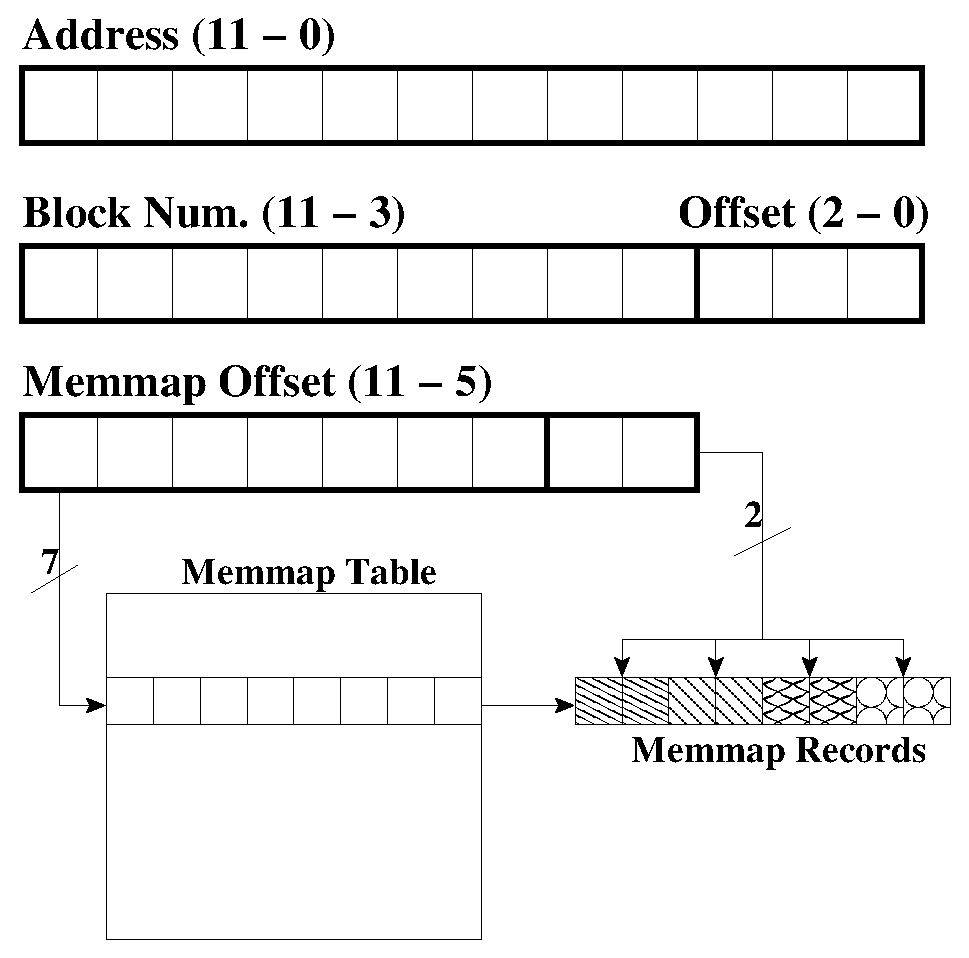
\includegraphics[height=2.5in, keepaspectratio=true]{figures/memaddrtrans.eps} 
%    \caption{Address to memory map translation (Two Domain Mode)}
%    \label{fig:addr_memmap_translate}
% \end{figure}
% %
% % If we optimize the memory map table to not include certain portions of the address space, then what will happen if we accidentally pass an unmapped address ?
% %
% %
% %
% \begin{table}[htdp]
%    \centering
%    \small{
%    \begin{tabular}{|l|l|}
%    \hline
%    Prototype & Description \\
%    \hline
%    int8\_t memmap\_set(uint8\_t blkID, uint8\_t nBlks,& Set owner of segment\\
%    uint8\_t domID) & [BlkID, BlkID + nBlks) to domID \\
%    \hline
%    uint8\_t memmap\_get(uint8\_t blkID) & Get owner and layout\\
%    & of block number BlkID \\
%    \hline
%    \end{tabular}
%    }
%    \centering
%    \caption{Memory Map API}
%    \label{tab:memmap_api}
% \end{table}
% %
% %
% %========================================================================================================================================
% % MEMORY MAP FOR PROTECTION
% %========================================================================================================================================
% \section{Using Memory Map For Protection}
% \label{subsec:mmap_for_protection}
% %
% Information stored in memory map data-structure can be used for creating a variety of protection models;
% %
% our protection model restricts programs from writing to memory outside their domain.
% %
% We discuss how memory map can be used in any system to enforce this protection model.
% %



% %
% Systems using memory map need to ensure following four conditions.
% %
% First, memory map should accurately reflect current ownership and layout.
% %
% In any real system, memory is constantly allocated, de-allocated or transferred from one module to another.
% %
% Memory map should be immediately updated when any of these events occur.
% %
% For example in SOS, \texttt{malloc}, \texttt{free} and \texttt{change\_own} system calls were modified to update memory map data structure. 
% %
% Second, only block owner should be permitted to free or change its ownership.
% %
% This condition is necessary as one module may accidentally (due to programming errors) free up memory that is being used by other module in the system.
% %
% Also it prevents a module from accidentally hijacking memory that is owned by other modules.
% %
% To enforce this condition, system needs to track the current active domain.
% %
% We describe implementation details of tracking current active application in Section~\ref{sec:cfmgr}.
% %
% Third, access to memory map API (described in Table ~\ref{tab:memmap_api}), should be restricted to single trusted domain.
% %
% If modules are allowed direct access to memory map API, then we can no longer trust information stored in it.
% %
% Programming bugs can cause incorrect parameters to be passed to memory map API.
% %
% In SOS, kernel is treated as a trusted domain and is allowed access to memory map API.
% %
% User modules are prevented access by restricting their control flow.
% %
% Fourth, blocks storing memory map data structure should be owned by the trusted domain.
% %
% This condition prevents accidental corruption of memory map data structure.
% %


% %The memory map manager tracks the permission information for every block in the address space of the sensor node.
% %
% Memory map can be easily incorporated into software systems.
% %
% As an example, we describe usage of memory map in SOS operating system to provide two domain (User-Kernel) protection.
% %
% %Memory map Two domain protection in SOS is easily implemented.
% %
% Memory map is initialized such that all statically allocated kernel memory blocks in address space are marked as owned by kernel.
% %
% Statically allocated blocks are used exclusively by kernel only and user modules never read or write to them.
% %
% Remaining portion of address space is partitioned into heap and a stack.
% %
% Heap is divided into blocks and a set of contiguous blocks (segments) are dynamically allocated to user modules or the kernel upon request.
% %
% Hence, minimum granularity of memory allocation is a block.
% %
% % Mention something about the choice of block size
% %
% Memory map for heap is initially marked as Free.
% %
% Stack has no memory map.
% %
% We discuss stack protection in Section~\ref{subsec:stackguard}.
% %
% Our implementation modified only 150 lines of code out of 12720 lines in SOS kernel.
% %
% This represents about 1\% change and most of it is localized to dynamic memory management routines. 
% %
% %
% % What are the implications of over-writing the stack ?


% %
% %The memory map manager works closely with the dynamic memory manager in the SOS operating system.
% %
% %Any request for dynamic memory is passed to the memory map manager that sets the correct permissions for the set of allocated blocks.
% %
% %During free operation, the memory map manager automatically clears the permissions.
% %
% %The dynamic memory manager in SOS permits the ownership change for dynamically allocated memory blocks.
% %
% %The memory map manager tracks any changes to the permissions that are caused due to the ownership transfer of a set of memory blocks.
% %
% %
% %
% %The dynamic memory allocator in SOS maintains a free list of unused memory blocks.
% %
% %Figure~\ref{fig:sos_free_list} shows the data structure implementing a memory block in SOS kernel.
% %
% %The data structure contains meta-data that stores the number of contiguous blocks constituting the current segment.
% %
% %This information is critical for the correct functioning of the dynamic memory allocator.
% %
% %However, as the meta-data is a part of the memory block, it can be easily corrupted by the user module.
% %
% %This is because the protection is provided only at the block level granularity.
% %
% %The problem was solved by eliminating the meta-data information from the block structure and deriving it at run-time based upon the layout information stored in the memory map table.
% %
% %The absence of the meta-data impacts the execution overhead of the dynamic memory operations.
% %
% %
% %========================================================================================================================================
% % MEMORY MAP CHECKER
% %========================================================================================================================================
% \section{Memory Map Checker}
% %
% A run-time checker is required to validate memory accesses made by software components.
% %
% Memory accesses need to be validated against a protection model.
% %
% Our memory map checker enforces the protection model that we described earlier; programs can write only into their domain.
% %
% Further, a single trusted domain in the system is allowed to access all memory.
% %
% Memory map checker belongs to the trusted domain.
% %
% %A run-time checker restricts the memory access of user modules to permissible regions.
% %
% %The access control permissions are stored and tracked by the memory map manager.
% %
% %The policy used for access control can vary.
% %
% %The most common policy is to prevent the user modules from ever writing to a memory region that is owned by the kernel.
% %
% %The modules are instrumented to introduce checks before every write operation that needs protection.
% %
% %   // Get permissions through bit shifts
%  %  // uint8_t perms_bm = (BLOCK_TYPE_BM << ((mmap_offset >> 3) << 1));
% Pseudo-code for write access checks is shown in Figure~\ref{fig:checker}.
% %
% \begin{figure} [h]
%   \centering
%     {\small
% \begin{verbatim}
% WRITE_ACCESS_CHECK(addr_t addr){
%   // Check is for writes outside stack region
%   if (addr < STACK_PTR){
  
%    // Retrieve permissions byte
%    uint16_t  mmap_index = (addr >> 5);
%    uint8_t   perms = MEM_MAP_PERMS_TBL[mmap_index];
  
%    // Generate bit mask
%    uint8_t   mmap_offset = (addr & 0x1f);
%    // Get permissions through look-up table
%    uint8_t   perms_bm = MEM_MAP_BM_LUT[mmap_offset];
   
%    // Check validity
%    if  !(perms & perms_bm) mem_access_exception();
%   } 
%  // Check for writes to stack 
%  else{
%    stack_access_check(addr);
%  } 
% }
% \end{verbatim} }
%   \caption{Pseudo-code for memory map checker (For two-domain protection)}
%   \label{fig:checker}
% \end{figure}

% %
% The write access checker performs three operations.
% %
% First, it retrieves the byte containing ownership information from memory map table for a given address.
% %
% Second, it generates a bit mask from the address offset to derive the actual permission.
% %
% Third, it checks the permission and signals memory access violation for invalid operations.
% %
% Algorithm to retrieve the permissions byte from memory map has already been discussed in Figure~\ref{fig:addr_memmap_translate}.
% %
% Generation of the bit mask requires complex bit shift operations.
% %
% These operations require 32 clock cycles on Atmega128L as there is no instruction level support for arbitrary bit shifts.
% %
% Therefore, a lookup table is used; this is stored in flash memory to minimize RAM usage.
% %
% Organization of the lookup table and its operation is described in Figure~\ref{fig:perm_lut}.
% %
% The lookup table takes only 8 clock cycles.
% %
% Therefore, the checker is designed to introduce minimal execution overhead.
% %
% The sub-routine is optimized for specific processor architecture to maximize efficiency.
% %
% %For example, the micro-controller architecture such as the Atmega128L does not have instruction level support for arbitrary bit shifts.
% %
% %
% As mentioned previously, the memory map manager does not maintain permissions for run-time stack.
% %
% Therefore, all write accesses to the stack are subject to a different check that will be discussed later.
% %
% % \begin{figure}[htbp]
% %   \centering
% %    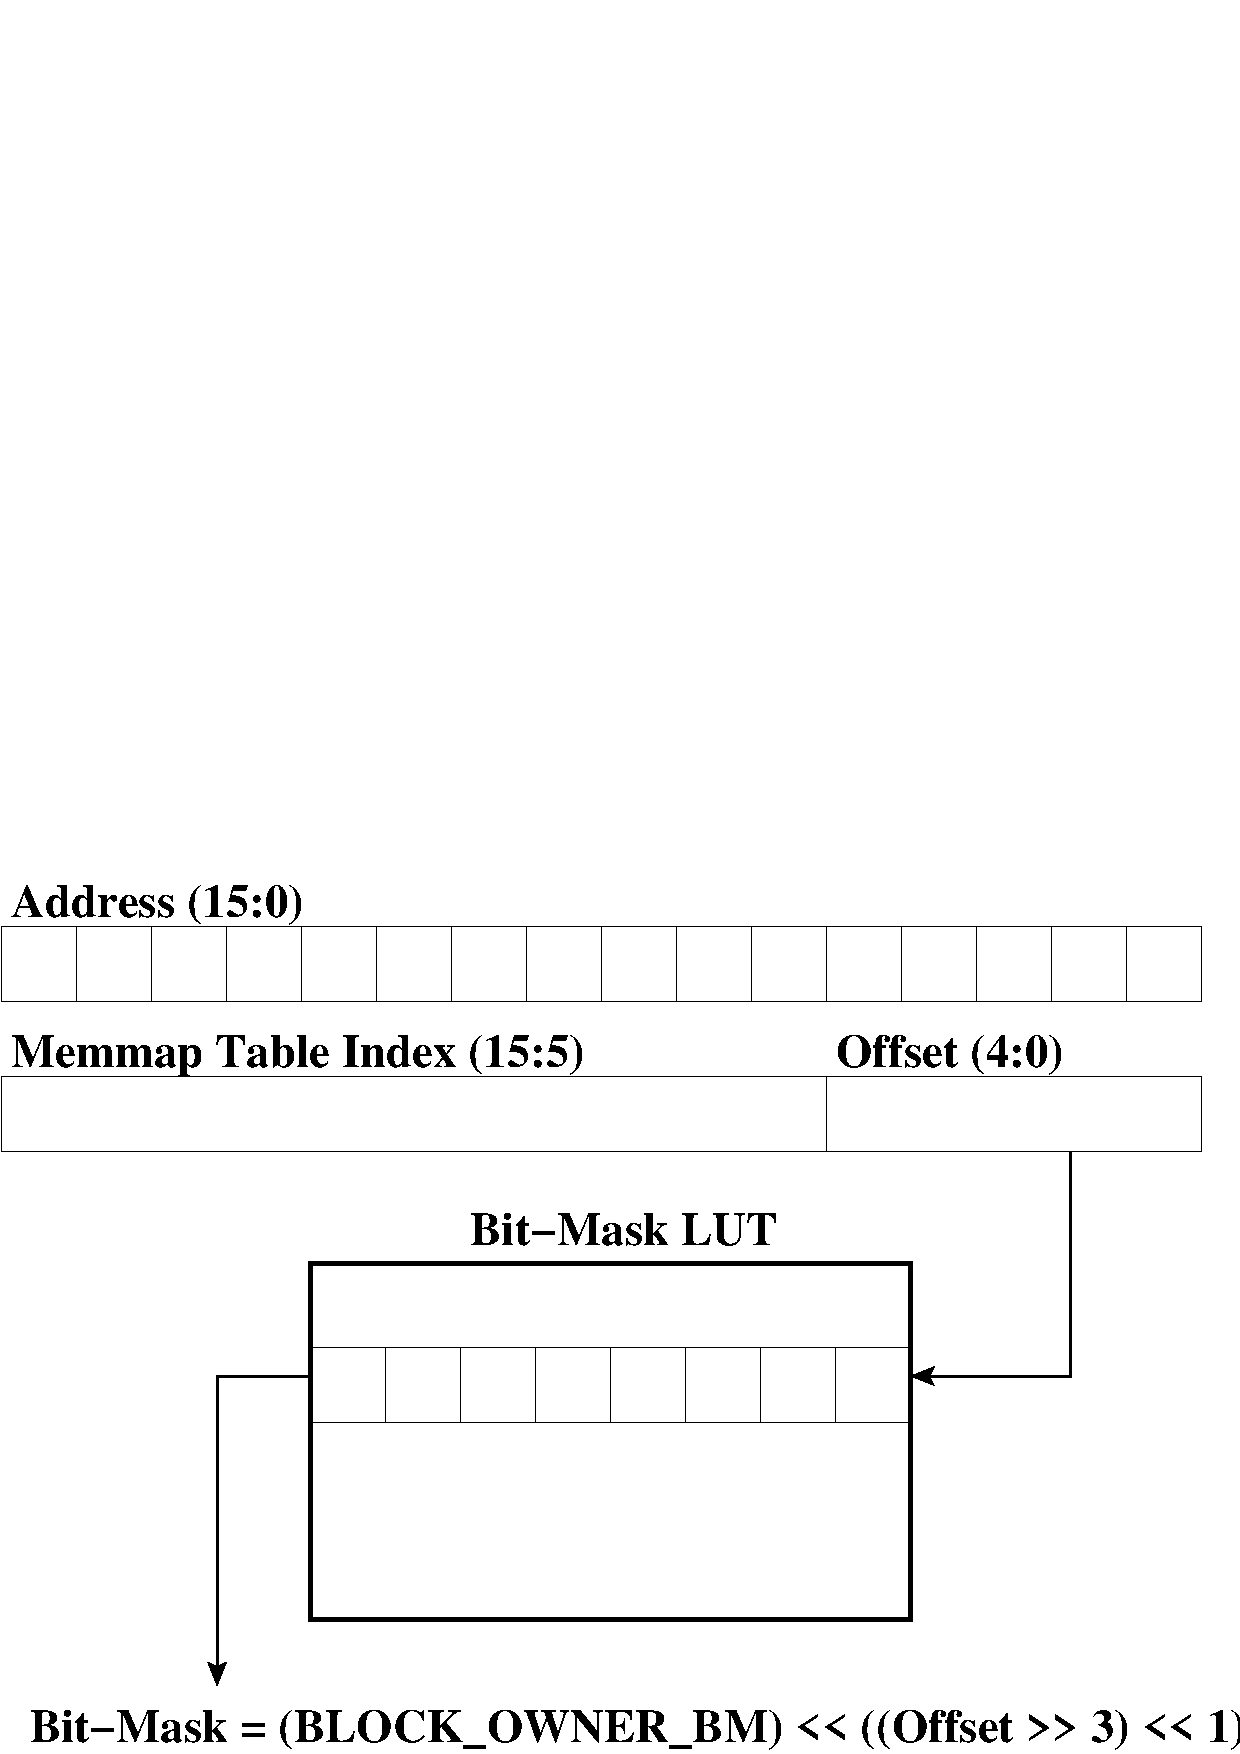
\includegraphics[height=2.5in, keepaspectratio=true]{figures/perms_lut_opt.jpg} 
% %    \caption{Lookup table optimization to implement bit-shit operations}
% %    \label{fig:perm_lut}
% % \end{figure}
% %
% %========================================================================================================================================
% % MEMORY HEAP META-DATA
% %========================================================================================================================================
% \section{Memory Heap Meta-data}
% %
% This section describes a practical issue that is faced while using memory map with heaps used for dynamic memory allocation.
% %
% Applications running on embedded micro-controllers share a single heap.
% %
% This is unlike desktop systems where each process has its own heap.
% %
% Heap implementations store meta-data information in data-structures that are embedded within allocated memory.
% %
% %For example, SOS kernel implements ownership tracking of memory segments.
% %
% %During module unloading, kernel uses the ownership information to free all memory owned by that module.
% %
% For example, SOS kernel stores segment size as meta-data within first memory block of segment as shown in Figure~\ref{fig:sos_free_list}.
% %
% This organization enables the heap to efficiently reclaim memory that is freed.
% %
% %The segment size information is used to implement the dynamic memory allocate and free routines.
% %
% However, modules can overwrite the meta-data as it lies within block boundary.
% %
% Recall, that permissions are stored only at block granularity.
% %
% Therefore, memory map checker is modified such that the meta-data in the first block of any segment is protected from writes.
% %
% Note that memory map table maintains layout information that identifies the starting block of any segment.
% %
% Additional checks are also implemented using look-up table for improved efficiency.
% %
% \begin{figure} [h]
%   \centering
%     {\small
% \begin{verbatim}
% typedef struct _Block
% {
%   uint16_t segmentSize;
%   union
%   {
%     uint8_t userPart[BLOCK_SIZE - sizeof(uint16_t)];
%     struct 
%     {
%       struct _Block *prev;
%       struct _Block *next;
%     };
%   } ;
% } Block;
% \end{verbatim} }
% \caption{Block implementation in SOS kernel}
% \label{fig:sos_free_list}
% \end{figure}


% %
% %Checks are introduced by a re-write of binary generated by cross-compiler tool-chain.
% %
% %We describe design of binary rewriter in Section~\ref{sec:writeverify}
% %
% %The CIL (C Intermediate Language)~\cite{cil02necula} framework catches all the writes made by the user module and inserts the appropriate write access check.
% %
% %In future, the checks would be introduced by an automatic binary re-write of the user modules.
% %
% %The binary re-writes would be performed at the load time of the modules into the sensor network.
















